\documentclass{article}
\usepackage[utf8]{inputenc}
\usepackage{graphicx}

\begin{document}
\title{Day 5}

\author{\emph{Teemu Sarapisto}}
\maketitle

\newcommand{\aaa}[3]{%
  \fbox{\includegraphics[height=30mm]{#1}} \quad
  \fbox{\includegraphics[height=30mm]{#2}} \quad
  \fbox{\includegraphics[height=30mm]{#3}} \par}
\newcommand{\bbb}[3]{%
  \medskip\noindent\aaa{#1}{#1-#2}{#1-#3}}

\newpage

\setlength{\fboxsep}{0pt}%

\section{Hands-on}

\subsection{StereoBM\_create}
\begin{figure}[h]
    \centering
    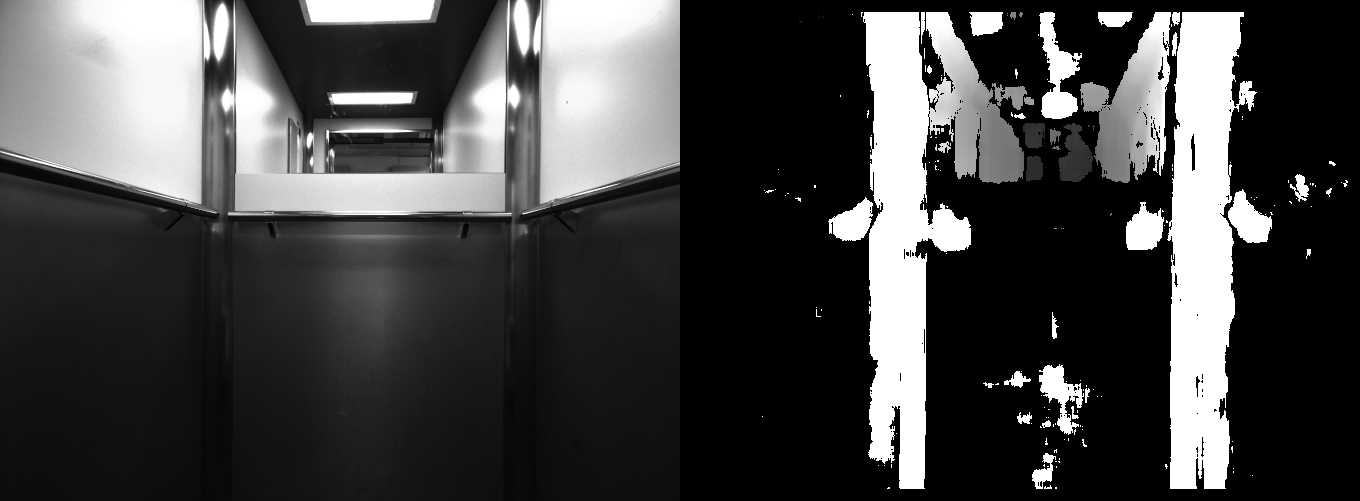
\includegraphics[scale=0.30]{StereoBM_create}
\end{figure}
\begin{verbatim}
import numpy as np
import cv2
from matplotlib import pyplot as plt

stereo = cv2.StereoBM_create(numDisparities=64, blockSize=25)
disparity = stereo.compute(imgL, imgR)
combod = np.concatenate((imgL, disparity), axis=1)
#plt.imsave('SGBM.png', combod)
#plt.imshow(combod)
#plt.show()

for frame in np.arange(40, 999, 2):
    fL = str(frame).zfill(8)
    fR = str(frame + 1).zfill(8)
    filenameL = "frames/%s.jpeg" % fL
    filenameR = "frames/%s.jpeg" % fR
    print(filenameL)
    print(filenameR)
    imgL = cv2.imread(filenameL, 0)
    imgR = cv2.imread(filenameR, 0)
    disparity = stereo.compute(imgL, imgR)
    print(disparity)
    np.amax(disparity)
    combod = np.concatenate((imgL, disparity), axis=1)
    print()
    cv2.imshow('ses', combod / 255)
    cv2.imwrite('StereoBM_create.png', combod)
    exit()
    cv2.waitKey(1)
\end{verbatim}
\subsection{StereoSGBM\_create}
\begin{figure}[h]
    \centering
    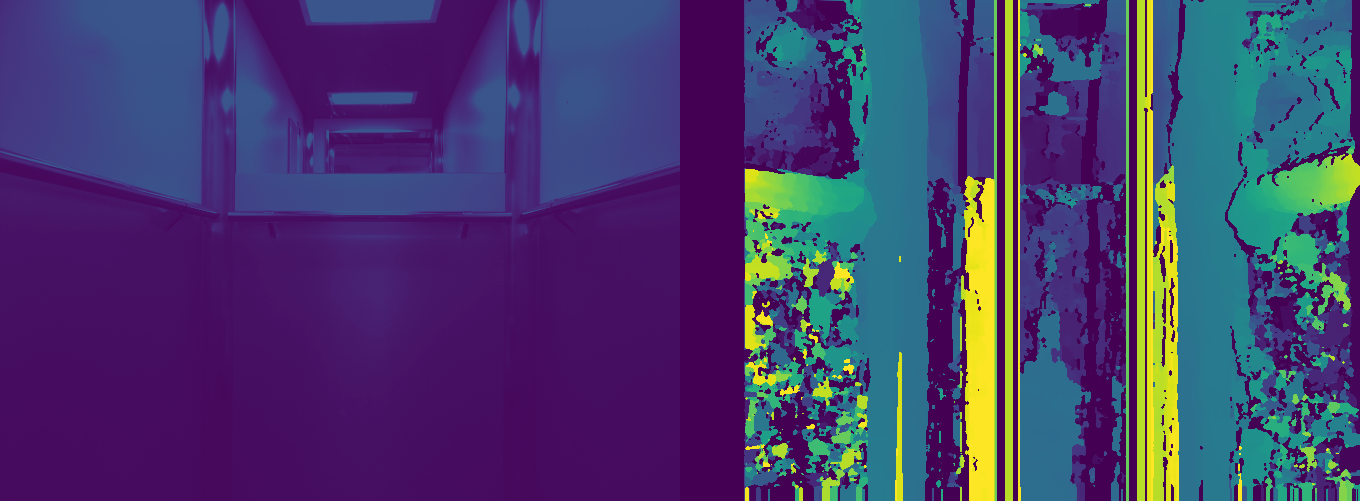
\includegraphics[scale=0.30]{SGBM}
\end{figure}
Code is about the same as for BM
\subsection{Study creation of optical flow fields with calcOpticalFlowPyrLK()}
\begin{figure}[h]
    \centering
    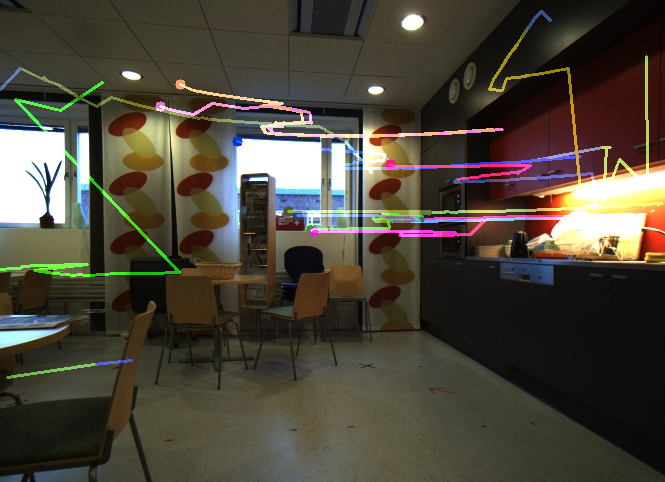
\includegraphics[scale=0.60]{optical_flow_pyrlk}
\end{figure}

\begin{verbatim}
feature_params = dict( maxCorners = 100,
                       qualityLevel = 0.3,
                       minDistance = 7,
                       blockSize = 7 )

lk_params = dict( winSize  = (15,15),
                  maxLevel = 2,
                  criteria = (cv2.TERM_CRITERIA_EPS | cv2.TERM_CRITERIA_COUNT, 10, 0.03))

fL = str(0).zfill(8)
fR = str(1).zfill(8)
filenameL = "frames/%s.jpeg" % fL
#filenameR = "frames/%s.jpeg" % fR
old_imgL = cv2.imread(filenameL, 0)
old_img_color = cv2.imread(filenameL)
#old_imgR = cv2.imread(filenameR, 0)

color = np.random.randint(0, 255, (100, 3))

mask = np.zeros_like(old_img_color)

p0 = cv2.goodFeaturesToTrack(old_imgL, mask = None, **feature_params)

for frame in np.arange(2, 999, 2):
    fL = str(frame).zfill(8)
    #fR = str(frame + 1).zfill(8)
    filenameL = "frames/%s.jpeg" % fL
    #filenameR = "frames/%s.jpeg" % fR
    print(filenameL)
    img_color = cv2.imread(filenameL)
    imgL = cv2.imread(filenameL, 0)

    p1, st, err = cv2.calcOpticalFlowPyrLK(old_imgL, imgL, p0, None, **lk_params)

    # Select good points
    good_new = p1[st==1]
    good_old = p0[st==1]
    # draw the tracks
    for i,(new,old) in enumerate(zip(good_new,good_old)):
        a,b = new.ravel()
        c,d = old.ravel()
        mask = cv2.line(mask, (a,b),(c,d), color[i].tolist(), 2)
        img_color = cv2.circle(img_color,(a,b),5,color[i].tolist(),-1)

    print(img_color.shape)
    print(mask.shape)
    img = cv2.add(img_color, mask)
    # Now update the previous frame and previous points
    old_imgL = imgL.copy()
    good_new_reshape = good_new.reshape(-1,1,2)

    if len(good_new_reshape) == 0:
        print('derp')
        p0 = cv2.goodFeaturesToTrack(old_imgL, mask = None, **feature_params)
        mask = np.zeros_like(old_img_color)
    else:
        p0 = good_new_reshape
        
    cv2.imshow('ses', img)
    cv2.waitKey(int(1000/70))
\end{verbatim}

\subsection{Use function  calcOpticalFlowFarneback() to do dense optical flow tracking}
\fbox{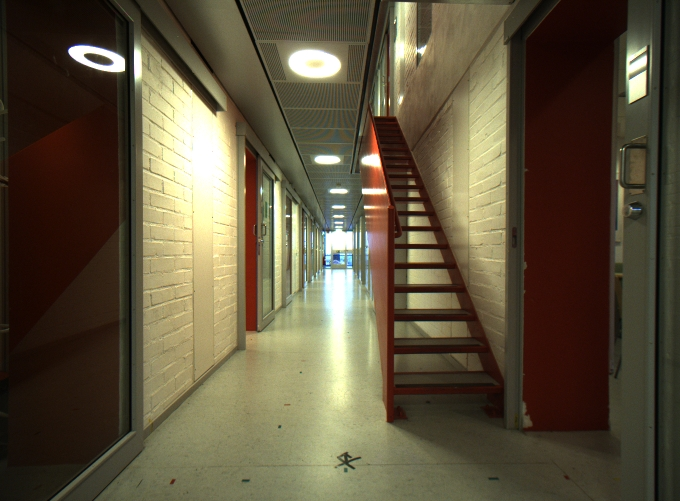
\includegraphics[scale=0.35]{opticalfb}} \quad
\fbox{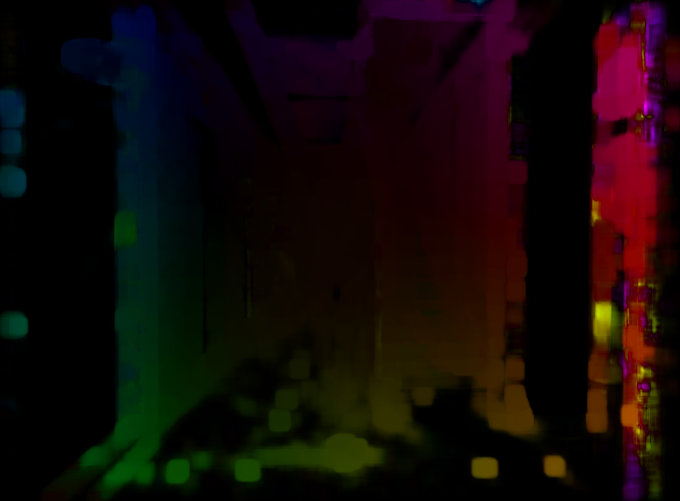
\includegraphics[scale=0.35]{opticalhsv}} \quad

\begin{verbatim}
def get_frame(n):
    fL = str(n).zfill(8)
    filenameL = "frames/%s.jpeg" % fL
    print(filenameL)
    img_color = cv2.imread(filenameL)
    imgL = cv2.imread(filenameL)
    return imgL, img_color


frame1, color_f1 = get_frame(0)
#frame1, color_f1 = get_frame(0)
print(frame1)

prvs = cv2.cvtColor(frame1, cv2.COLOR_BGR2GRAY)
hsv = np.zeros_like(frame1)
hsv[...,1] = 255

for frame_num in np.arange(2, 999, 2):
    frame2, color_f2 = get_frame(frame_num)

    next = cv2.cvtColor(frame2,cv2.COLOR_BGR2GRAY)
    flow = cv2.calcOpticalFlowFarneback(prvs,next, None, 0.5, 3, 15, 3, 5, 1.2, 0)
    mag, ang = cv2.cartToPolar(flow[...,0], flow[...,1])
    hsv[...,0] = ang*180/np.pi/2
    hsv[...,2] = cv2.normalize(mag,None,0,255,cv2.NORM_MINMAX)
    bgr = cv2.cvtColor(hsv,cv2.COLOR_HSV2BGR)
    cv2.imshow('frame2',bgr)
    k = cv2.waitKey(30) & 0xff
    if k == 27:
        break
    elif k == ord('s'):
        cv2.imwrite('opticalfb.png',frame2)
        cv2.imwrite('opticalhsv.png',bgr)
    prvs = next

\end{verbatim}

\subsection{How long it took}
around 4 hours


\end{document}
%  LocalWords:  Jorma Laaksonen pdf py tex OpenCV libopencv dev jpg
%  LocalWords:  highgui imgproc imgcodecs greyscale png opencv ing
%  LocalWords:  texlive includegraphics Exactum Gür Ersalan
